\documentclass{article}
\usepackage{graphicx}
%----------------------------------------------------------------------------------------
%	PACKAGES AND OTHER DOCUMENT CONFIGURATIONS
%----------------------------------------------------------------------------------------

\usepackage{amsmath,amsfonts,amssymb} % Math packages

\usepackage{enumerate} % Custom item numbers for enumerations

\usepackage{listings} % File listings, with syntax highlighting

%----------------------------------------------------------------------------------------
%	DOCUMENT MARGINS
%----------------------------------------------------------------------------------------

\usepackage{geometry} % Required for adjusting page dimensions and margins

\geometry{
	paper=a4paper, % Paper size, change to letterpaper for US letter size
	top=2.5cm, % Top margin
	bottom=3cm, % Bottom margin
	left=2.5cm, % Left margin
	right=2.5cm, % Right margin
	headheight=14pt, % Header height
	footskip=1.5cm, % Space from the bottom margin to the baseline of the footer
	headsep=1.2cm, % Space from the top margin to the baseline of the header
	%showframe, % Uncomment to show how the type block is set on the page
}

\usepackage[utf8]{inputenc} % Required for inputting international characters
\usepackage[T1]{fontenc} % Output font encoding for international characters
%\renewcommand{\familydefault}{\sfdefault}
 % Include the file specifying the document structure and custom commands

%----------------------------------------------------------------------------------------
%	ASSIGNMENT INFORMATION
%----------------------------------------------------------------------------------------

\title{Econometrics: Homework} % Title of the assignment

\author{Caio Figueiredo} % Author name and email address

%----------------------------------------------------------------------------------------

\begin{document}

\maketitle % Print the title

%----------------------------------------------------------------------------------------
%	PROBLEM 1
%----------------------------------------------------------------------------------------

\section{Question 2}

\subsection{a}

In the following graphs the kernel number 4 will be ignore, since it's MSE 
is much worse than the others that it undermines readability.

\begin{center}
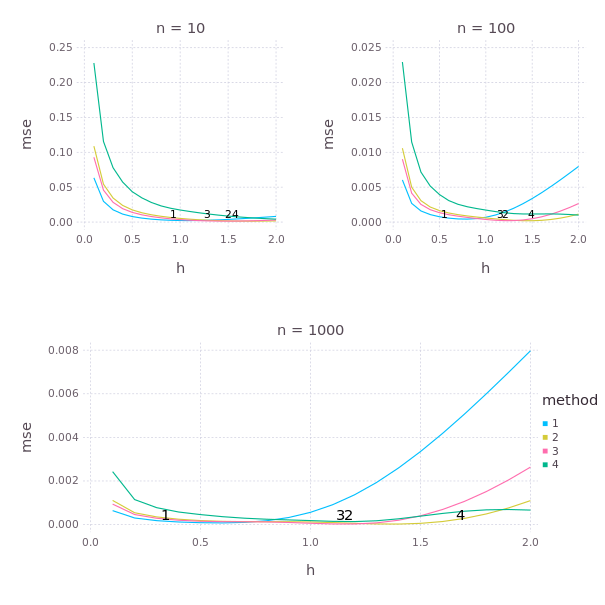
\includegraphics[width=16cm, height=16cm]{Q2-a.png}
\end{center}

The points 1,2 and 3 are the suggested value for the bandwidth using the cross
validation method for kernel number 1, 2 and 3 respectively. The method does not
match the value of $h$ that minimizes the $MSE$ but overall behave really well and stays
in a decently close neighborhood of that point.

\subsection{b}

\begin{center}
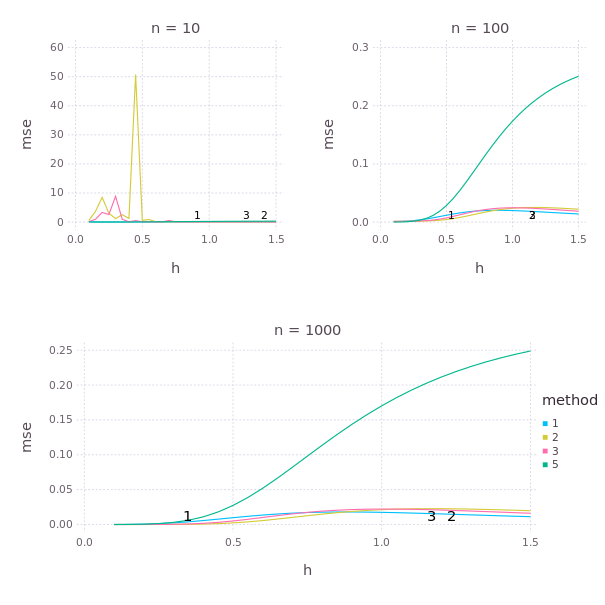
\includegraphics[width=16cm, height=16cm]{Q2-b.png}
\end{center}

Here we have a different story, ignoring the case for $n = 10$ where the our estimator
does not behave really well the $MSE$ seems to be a increasing function of the bandwidth,
that is the lower the $MSE$ the better, which is not at all that intuitive.

Of course because of this the values suggested by the cross validation method does not
work well if the regression estimator.

This graph also have an additional line (\#5) which reference the local linear estimator,
the $MSE$ of this line does not really compare to the other lines since we are estimating
different objects but the behavior along $h$ seems to be the same.

\section{3}



\end{document}
